\documentclass[a4paper, 11pt, ngerman, fleqn]{article}
\usepackage[utf8]{inputenc}
\usepackage{graphicx}
\usepackage{babel}
\usepackage{ngerman}
\usepackage{coordsys,logsys,color}
\usepackage{german,fancyhdr}
\usepackage{hyperref}
\usepackage{texdraw}
\input{txdtools}

\NeedsTeXFormat{LaTeX2e}
\ProvidesPackage{hyperref}
\definecolor{darkblue}{rgb}{0,0,.6}
\hypersetup{pdftex=false, colorlinks=true, breaklinks=true, linkcolor=darkblue, menucolor=darkblue, pagecolor=darkblue, urlcolor=darkblue, citecolor=darkblue}

\pagestyle{fancy}

%!TEX root = Pflichtenheft.tex
\renewcommand{\familydefault}{cmss}

\definecolor{fgcgray}{rgb}{0.4, 0.4, 0.4}
\definecolor{bgctitle}{rgb}{0.5, 0.5, 0.5}
\newcommand{\titlefont}[1]{\textcolor{bgctitle}{\fontfamily{cmss}\fontseries{bx}\fontshape{n}\fontsize{20.48}{0pt} \selectfont #1}}

\addtolength{\oddsidemargin}{-1.0cm}
\addtolength{\evensidemargin}{-1.0cm}
\addtolength{\headwidth}{2.0cm}
\addtolength{\textwidth}{2.0cm}

\setlength{\parindent}{0cm}

\newcommand{\spaceline}[1][8pt]{\vskip #1}
\newcommand{\comment}[1]{\spaceline[5pt] \textcolor{fgcgray}{\scriptsize #1} \spaceline[15pt]}
\newcommand{\attrname}[1]{\textcolor{fgcgray}{\scriptsize #1}}


\makeatletter

\newcommand*{\project}[1]{\gdef\@project{#1}}
\newcommand*{\tutor}[1]{\gdef\@tutor{#1}}
\newcommand*{\group}[1]{\gdef\@group{#1}}

\def\@maketitle{
	\begin{titlepage}
	\begin{center}
	
\includegraphics[width=0.5\textwidth]{TUC-Logo.jpg}\\
	Praktikum Softwareentwurf Wintersemester 2011/12\\
	\vspace{12em}
	\Large{Pflichtenheft} \\
	\vspace{1em}
	\Huge{\textbf{\@project}}
	\end{center}
	\vspace{20em}
	\begin{tabular}[t]{rl}
		\attrname{Gruppe:} & \@group \\
		\attrname{Autoren:} & \@author \\
		\attrname{Betreuer:} & \@tutor \\
		\attrname{letzte Änderung:} & \@date
	\end{tabular}

	\end{titlepage}
}

\setcounter{secnumdepth}{4}
\setcounter{tocdepth}{4}

\makeatother

\everytexdraw{
	\drawdim cm \linewd 0.01
	\arrowheadtype t:T
	\arrowheadsize l:0.2 w:0.2
	\setgray 0.5
}

\begin{document}
	%!TEX root = Pflichtenheft.tex

\title{Pflichtenheft Praktikum Softwareentwurf WS 2011/12}
\project{Rechnungssystem}
\author{Sascha Ebert () - Teamleiter\\&Morris Jobke ()\\&Markus Ast ()\\&Robert Schönherr ()\\&Michael Hertel ()}
\tutor{Dr. Frank Seifert}
\groupnumber{1}

\maketitle \newpage
	\tableofcontents \newpage
	%!TEX root = Pflichtenheft.tex

\section{Zielbestimmungen}



\subsection{Musskriterien}

\begin{itemize}
	\item Rechnungssystem für Selbständige, welches Endjahresbilanzen bzw. Gewinn-Verlust-Überschussrechnungen bereitstellt
	\item Rechnungen können im PDF-Format ausgegeben werden
	\item Anpassbare Rechnungs-PDFs durch vom Nutzer vorgegebene Latex oder HTML-Templates
	\item Erstellen und Verwalten von Rechnungs-Repositorys zum Verwalten der Rechnungen
	\item Bereitstellung eines GDK-Frontends
\end{itemize}

\subsection{Sollkriterien}

\begin{itemize}
	\item Ausgegebene Rechnungs-PDFs werden digital signiert
\end{itemize}

\subsection{Abgrenzungskriterien}

\begin{itemize}
	\item Rechnungssystem beachtet keine Steuern
	\item Rechnungssystem nicht für Unternehmen geeignet
\end{itemize} \newpage
	%!TEX root = Pflichtenheft.tex

\section{Produkteinsatz}


\subsection{Anwendungsbereiche}

Das Rechnungssystem soll Kleinunternehmern eine einfache und effiziente Verwaltung und Erstellung von Rechnungen ermöglichen. 

\subsection{Zielgruppen}

Das Projekt richtet sich an Kleinunternehmer, welche Rechnungen erstellen und verwalten müssen. 

Grundlegende Computerkenntnisse und auch grundlegende Kentnisse von HTML bzw. Latex sind, für die Erstellung eigener Templates, von Vorteil, aber nicht zwingend notwendig.

Des Weiteren soll eine Grundlage für weiterreichende Projekte geschaffen werden, welche von anderen Entwicklern genutzt werden kann.

\subsection{Systemvoraussetzungen, Hardware}
Es werden folgende Komponenten benötigt:
\begin{itemize}
	\item PC mit Linux-, oder Mac-Betriebssystem
	\item Editor oder ähnliche Anwendung zum Bearbeiten der Templates (optional? -> Standard-Templates?)
	\item TeX-Distribution (optional)
	\item Sqlite (optional)
\end{itemize}

\subsection{Betriebsbedingungen}
Die Anwendung soll sich nicht stark von den Betriebsbedingungen anderer typischer Verwaltungssoftware unterscheiden:

\begin{itemize}
	\item Betriebszeit: bei Bedarf
	\item wartungsfrei
	\item die Sicherung der Daten obliegt dem Nutzer
\end{itemize}
 \newpage
	%!TEX root = Pflichtenheft.tex

\section{Produktübersicht}

% \begin{itemize}
% 	\item UML-Diagramme zu den Use-Cases hinzufügen
% \end{itemize}

% Repo erstellen und konfigurieren (Template, Rechnungsnummern, ...)
% Rechnung ausfüllen und erstellen (PDF, HTML, ...)
% Verwaltung der Rechnungen (offene Rechnungen, Statistiken, Analsye...)

% [Benutzer]-(Rechnung anlegen)
% [Benutzer]-(Rechnungsstatus ausgeben)
% [Benutzer]-(Rechnungsattribute bearbeiten)
% [Benutzer]-(Rechnung rendern)
% [Benutzer]-(Template konfigurieren)
% [Benutzer]-(Rechnungen durchsuchen)
% [Benutzer]-(Rechnung löschen)
% (Rechnung anlegen)<(Rechnungsattribute eingeben)
% (Rechnungsattribute bearbeiten)<(Rechnungsattribute eingeben)
% (Template konfigurieren)<(Platzhalter eintragen)
% http://yuml.me/5ed27f7e

\begin{center}
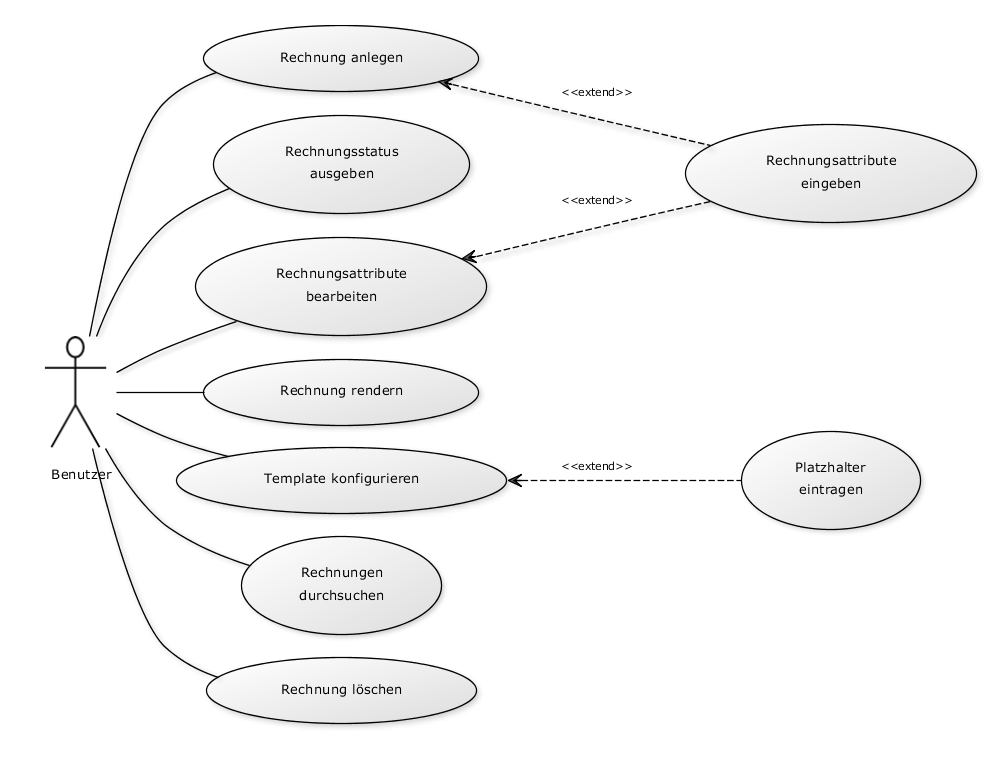
\includegraphics[width=0.8\textwidth]{03-Use-Case.png}
\end{center} \newpage
	%!TEX root = Pflichtenheft.tex

\section{Produktleistungen}

\begin{description}
	\item[/L100/]
		\textit{Genauigkeit:}
			Jegliche Geldbeträge im Programm sind auf 2 Nachkommastellen genau.
\end{description}

\begin{description}
	\item[/L200/]
		\textit{Unterstützung für korrekte Templates:}
			Verwendet der Programmnutzer ein unvollständiges Template mit fehlenden Platzhaltern erhält er eine Warnung.
\end{description}

\begin{description}
	\item[/L300/]
		\textit{Akkumulation:}
			Bei fehlerhaften Eingaben erhält der Benutzer eine aussagekräftige Fehlermeldung.
\end{description}

	%\item Validierung
 \newpage
	%!TEX root = Pflichtenheft.tex

\section{Benutzeroberfläche}

\subsection{Kommando-Struktur}
Die Kommando-Struktur der Benutzeroberfläche ist durch das Programm \emph{git} inspiriert\\
\\\\
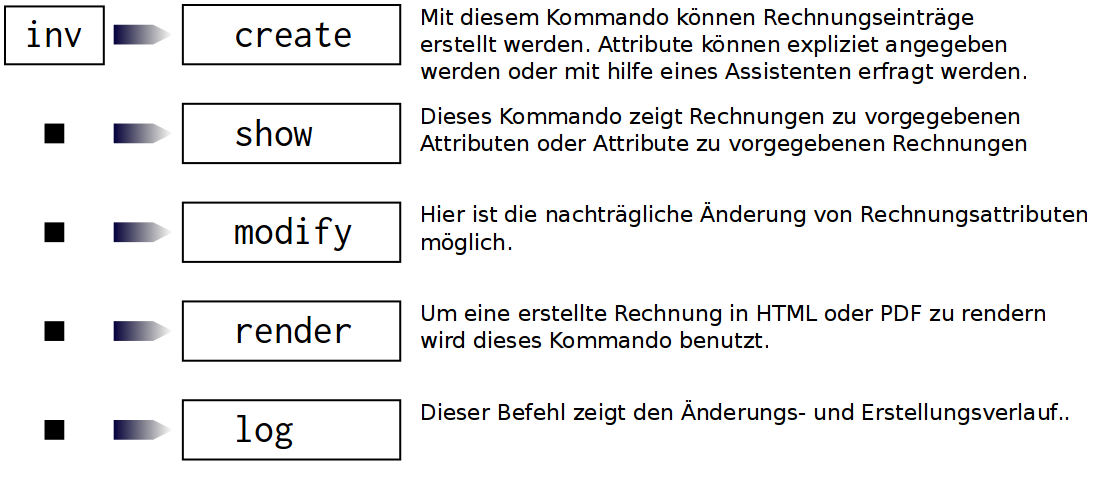
\includegraphics[width=\textwidth]{kommando-struktur.png}
\\
\subsection{Ordnerstruktur}
Es ist möglich mit der Ordnerstruktur innerhalb eines Repositories diverse
Standard-Attributwerte zu definieren. Dies geschieht im Zusammenhang mit den vom
Benutzer gewählten Ordnungsschlüsseln.\\
\\\\
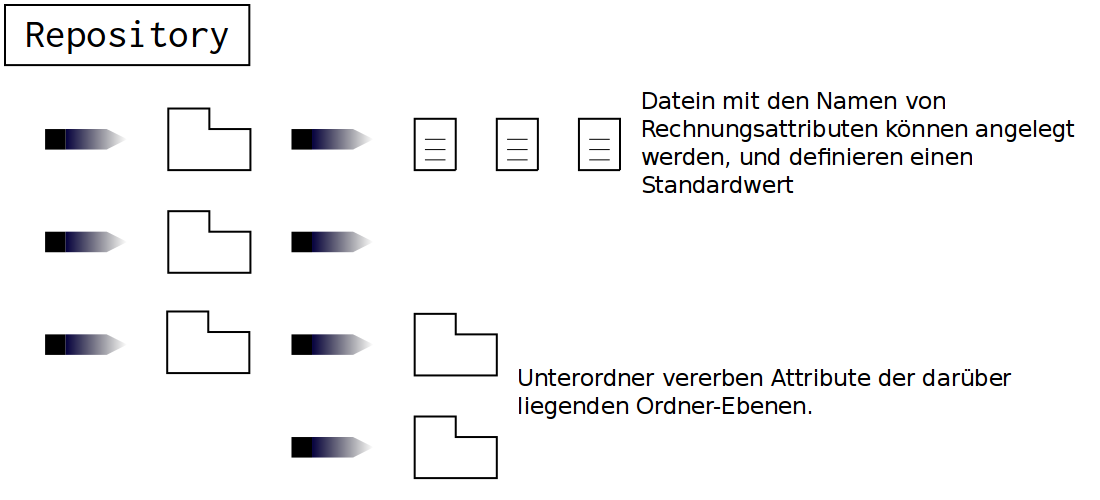
\includegraphics[width=\textwidth]{ordnerstruktur-struktur.png}
\\\\
\subsubsection*{Beispiel:}
Der Nutzer legt in seinem Rechnungsrepository jeweils einen Ordner für jeden Kunde
an. In jedem dieser Verzeichnisse plaziert er weiterhin eine Datei mit dem Namen
\emph{Adresse} worin er die Adresse des jeweiligen Kunden einträgt. Wenn er jetzt
im entsprechenden Kundenordner eine Rechnung kreiert ist das Attribut \emph{Adresse}
schon gesetzt.
 \newpage
	%!TEX root = Pflichtenheft.tex

\section{Qualitätsanforderungen}



\begin{center}
 \begin{tabular}{l|c|c|c|c}
  ~ & sehr wichtig & wichtig & weniger wichtig & unwichtig\\
  \hline \hline
  \textit{Robustheit}~ &  ~ ~ ~ & \textbf{X}~ &  ~ ~ ~ &  ~ ~ ~ \\
  \hline
  \textit{Zuverlässigkeit}~ & \textbf{X}~ &  ~ ~ ~ &  ~ ~ ~ &  ~ ~ ~ \\
  \hline
  \textit{Korrektheit}~ & \textbf{X}~ &  ~ ~ ~ &  ~ ~ ~ &  ~ ~ ~ \\
  \hline
  \textit{Benutzungsfreundlichkeit}~ &  ~ ~ ~ & \textbf{X}~ &  ~ ~ ~ &  ~ ~ ~ \\
  \hline
  \textit{Effizienz}~ &  ~ ~ ~  &  ~ ~ ~ & \textbf{X}~ &  ~ ~ ~ \\
  \hline
  \textit{Portierbarkeit}~ &  ~ ~ ~ &  ~ ~ ~ & \textbf{X}~ &  ~ ~ ~ \\
  \hline
  \textit{Kompatibilität}~ &  ~ ~ ~ & \textbf{X}~ &  ~ ~ ~ &  ~ ~ ~ \\
 \end{tabular}
\end{center}
 \newpage
	%!TEX root = Pflichtenheft.tex

\section{Testszenarien und Testfälle}



\begin{description}
  \item[/T0010/]
	\textit{Repository}
	\begin{description}
		\item[Ausgangszustand]
		Verzeichnis außerhalb eines bestehenden Repositories.
		\item[Aktion]
		Anlegen eines neuen Rechnungs-Repositorys mit \textit{inv init}.
		\item[Erwarteter Zielzustand]
		Valides Rechnungs-Repository im Zielverzeichnis.
	\end{description}

  \item[/T0020/]
	\textit{Erstellen}
	\begin{description}
		\item[Ausgangszustand]
		Vorhandenes Rechnungs-Repository.
		\item[Aktion]
		Erstellen einer neuen Rechnung mit \textit{inv create}.
		\item[Erwarteter Zielzustand]
		Erstellte Rechnung im Rechnungs-Repository.
	\end{description}

  \item[/T0030/]
	\textit{Auslesen}
	\begin{description}
		\item[Ausgangszustand]
		Vorhandenes Rechnungs-Repository mit vorhandener Rechnung.
		\item[Aktion]
		Auslesen einer Rechnung mit \textit{inv show}.
		\item[Erwarteter Zielzustand]
		Ausgabe der auszulesenden Rechnung.
	\end{description}

  \item[/T0040/]
	\textit{Bearbeiten}
	\begin{description}
		\item[Ausgangszustand]
		Vorhandenes Rechnungs-Repository mit vorhandener Rechnung.
		\item[Aktion]
		Verändern der Daten der Rechnung mit \textit{inv modify}.
		\item[Erwarteter Zielzustand]
		Aktualisierung der Daten im Repository.
	\end{description}

  \item[/T0050/]
	\textit{Löschen}
	\begin{description}
		\item[Ausgangszustand]
		Vorhandenes Rechnungs-Repository mit vorhandener Rechnung.
		\item[Aktion]
		Löschen der Rechnung im Repository mit \textit{inv remove}.
		\item[Erwarteter Zielzustand]
		Rechnung nicht mehr im Repository vorhanden.
	\end{description}

  \item[/T0060/]
	\textit{Rechnungsnummer-Syntax}
	\begin{description}
		\item[Ausgangszustand]
		Rechnungsnummer-Syntax mit enthaltenem Platzhalter für Jahr, Monat, Tag und den Teil der fortlaufenden Nummer.
		\item[Aktion]
		Generieren mehrere Rechnungen mit sich in Jahr, Monat und Tag unterscheidenden Datums.
		\item[Erwarteter Zielzustand]
		Die Jahr, Monat und Tag Platzhalter entsprechen dem angegeben Datum und die fortlaufende Nummer erhöht sich bei weiteren neugenerierten Rechnung immer nur dann, wenn es schon Rechnungen mit identischen Platzhalter Werten gibt. Dabei erhöht sich die fortlaufende Nummer um die Anzahl der bereits mit diesen Werten der Platzhalter generierten Rechnungen plus eins.
	\end{description}

  \item[/T0070/]
	\textit{Latex-Template}
	\begin{description}
		\item[Ausgangszustand]
		Vorhandenes Repostory mit Beispielrechnung und vorhandenes Latex-Template.
		\item[Aktion]
		Rechnung auf Basis des Latex-Templates generieren (mit \textit{inv render}).
		\item[Erwarteter Zielzustand]
		Latex-Datei, in der die Platzhalter durch die Parameter der Rechnung ersetzt oder bei nicht vorhanden Werten entfernt wurden.
	\end{description}

  \item[/T0080/]
	\textit{HTML-Template}
	\begin{description}
		\item[Ausgangszustand]
		Vorhandenes Repostory mit Beispielrechnung und vorhandenes HTML-Template.
		\item[Aktion]
		Rechnung auf Basis des HTML-Templates generieren (mit \textit{inv render}).
		\item[Erwarteter Zielzustand]
		HTML-Datei, in der die Platzhalter durch die Parameter der Rechnung ersetzt oder bei nicht vorhanden Werten entfernt wurden.
	\end{description}
\end{description}
 \newpage
	%!TEX root = Pflichtenheft.tex

\section{Entwicklungsumgebung}


\subsection{Software}

\begin{itemize}
  \item Plattform
    \begin{itemize}
		\item (Ubuntu) Linux, C++ (Version?), Latex (Version?), HTML (Version?)
    \end{itemize}
  \item Tools
    \begin{itemize}
  		\item Miktex 2.9, Editoren?
    \end{itemize}

\end{itemize}

\subsection{Hardware}

\begin{itemize}
	\item PCs
\end{itemize}

\subsection{Orgware}

\begin{itemize}
  	\item Git, Github
\end{itemize}
 \newpage
%   %!TEX root = Pflichtenheft.tex

\section{Ergänzungen}
 \newpage
	%!TEX root = Pflichtenheft.tex

\section{Glossar}


\begin{itemize}
	\item Template = eine Mustervorlage bei der in dafür vorgesehene Bereiche Daten eingefügt werden können
	\item Repository = ein verwaltetes Verzeichnis in welchem digitale Daten gespeichert werden können
	\item ...?
\end{itemize}


\end{document}
